\documentclass[11pt,a4paper]{article}

% ----------------------------------------------------------------------
%  Codificación e idioma
% ----------------------------------------------------------------------
\usepackage[utf8]{inputenc}
\usepackage[T1]{fontenc}
\usepackage{babel}
\babelprovide[import, main]{spanish}

% ----------------------------------------------------------------------
%  Matemática
% ----------------------------------------------------------------------
\usepackage{amsmath,amssymb,amsfonts}
\usepackage{mathtools}
\usepackage{bm}

% ----------------------------------------------------------------------
%  Tipografía, layout y enlaces
% ----------------------------------------------------------------------
\usepackage[a4paper,margin=2.4cm]{geometry}
\usepackage[protrusion=true,expansion=false]{microtype}
\usepackage{setspace}
\onehalfspacing
\setlength{\emergencystretch}{3em}
\usepackage{booktabs}
\usepackage{array}
\usepackage{longtable}
\usepackage{enumitem}
\usepackage{titlesec}
\usepackage{fancyhdr}
\usepackage{abstract}
\usepackage{float}
\usepackage[round,authoryear]{natbib}
\usepackage{caption}
\captionsetup{font=small,labelfont=bf}
\usepackage[dvipsnames,table]{xcolor}
\definecolor{kairosblue}{RGB}{0,0,0}
\usepackage{pgfplots}
\usepackage{booktabs}
\usepackage{tabularx}
\pgfplotsset{compat=1.16}
\usepackage[colorlinks=true,linkcolor=black,citecolor=black,urlcolor=black,
  pdftitle={Modelo Kairos: descriptor de estado fisiologico},
  pdfauthor={Juan Pablo Gelmi Garrido},
  pdfsubject={Informe tecnico-cientifico del modelo Kairos}]{hyperref}

% Encabezados de sección
\titleformat{\section}{\normalfont\large\bfseries\color{black}}{\thesection}{0.6em}{}
\titleformat{\subsection}{\normalfont\normalsize\bfseries\color{black}}{\thesubsection}{0.6em}{}
\titleformat{\subsubsection}{\normalfont\normalsize\itshape}{\thesubsubsection}{0.6em}{}

\pagestyle{fancy}
\fancyhf{}
\renewcommand{\headrulewidth}{0.3pt}
\lhead{\small\textit{Kairós — Documentación técnica del modelo}}
\rhead{\small\thepage}

% Operadores y abreviaturas
\DeclareMathOperator{\sgn}{sgn}
\DeclareMathOperator{\clamp}{clamp}
\DeclareMathOperator{\med}{med}
\DeclareMathOperator{\Var}{Var}
\DeclareMathOperator*{\argmax}{arg\,max}
\newcommand{\E}{\mathbb{E}}
\renewcommand{\refname}{Referencias bibliográficas}

\title{\vspace{-1.2cm}\bfseries\color{black}
Modelo Kairós: descriptor de estado fisiológico\\ para un corredor de media y larga distancia\\[4pt]
\large\normalfont\color{black}
Fundamentos teóricos y\\ metodología del sistema implementado}

\author{Juan Pablo Gelmi Garrido}
\date{\today}

\begin{document}
\maketitle
\thispagestyle{fancy}

\begin{abstract}
\noindent
Kairós es un modelo computacional de monitorización fisiológica diseñado para describir el estado de un corredor de media y larga distancia a partir de archivos de actividad. El sistema constituye un descriptor de estado fisiológico y no un predictor de rendimiento futuro. Su salida central es la \emph{carga y trayectoria de forma} del atleta: la carga crónica $g(t)$, la carga aguda $h(t)$, el balance de estrés $\mathrm{TSB}(t)$, el índice de \emph{momentum} de forma $\Pi_{\mathrm{rel}}(t)$ y el odómetro de nivel durable $\Pi_{\mathrm{abs}}(t)$, junto con los acumuladores de carga por dominio aeróbico y de alta intensidad $g_{\mathrm{aer}}$ y $g_{\mathrm{hii}}$. A esta familia de descriptores se añaden dos marcadores biomecánicos de fatiga intrasesión: la deriva del tiempo de contacto con el suelo (\emph{GCT drift}) y la recuperación de la frecuencia cardíaca tras el esfuerzo. Todas las magnitudes derivadas se calibran respecto de la propia distribución histórica del deportista mediante un enfoque estrictamente intraindividual. El informe presenta las variables de entrada, las variables derivadas, los parámetros y supuestos del sistema, junto con su formulación matemática y la justificación fisiológica, biomecánica y estadística de cada componente, así como sus limitaciones y condiciones de validez. El sistema no imputa señal cuando los datos de una sesión son insuficientes, de modo que ningún descriptor se fabrica sobre información ausente.

\vspace{4pt}
\noindent\textbf{Palabras clave:} monitorización del entrenamiento; descriptor de estado fisiológico; carga de entrenamiento; modelo fitness--fatiga; calibración intraindividual; deriva del tiempo de contacto; recuperación cardíaca.
\end{abstract}


\newpage
\tableofcontents
\vspace{0.4cm}
\hrule
\vspace{0.4cm}

% ======================================================================
\newpage
\section{Resumen ejecutivo}
% ======================================================================

Kairós es un sistema de modelado fisiológico de propósito único, construido para describir el estado de un corredor de resistencia con base exclusivamente en señales que ese atleta puede registrar de forma fiable y sostenida en el tiempo. El sistema toma como entrada archivos de actividad con series temporales de frecuencia cardíaca (FC), velocidad y dinámica de carrera. A partir de ellas deriva una familia de descriptores de \textbf{carga y trayectoria de forma}: mediante un modelo impulso-respuesta de medias móviles exponenciales (EWMA) se estiman la carga crónica $g(t)$ (\emph{fitness}), la carga aguda $h(t)$ (\emph{fatiga}) y el balance de estrés $\mathrm{TSB}(t)$ (\emph{frescura}), junto con un índice de \emph{momentum} de la carga crónica, $\Pi_{\mathrm{rel}}(t)$, y un odómetro acumulado de nivel durable, $\Pi_{\mathrm{abs}}(t)$. La misma carga se reparte en dos dominios fisiológicos, aeróbico y de alta intensidad, dando lugar a los acumuladores $g_{\mathrm{aer}}$ y $g_{\mathrm{hii}}$. Para cada día, estos son los descriptores de estado que el sistema afirma producir.

A ellos se suman dos marcadores biomecánicos de fatiga calculados \emph{dentro} de cada sesión: la deriva del tiempo de contacto con el suelo (\emph{GCT drift}), que cuantifica la degradación de la técnica a lo largo del esfuerzo, y la recuperación de la frecuencia cardíaca tras el esfuerzo, indicador de la reactivación parasimpática.

% ======================================================================
\section{Introducción y motivación}
\label{sec:motivacion}
% ======================================================================

La monitorización cuantitativa del entrenamiento busca representar, a partir de señales medibles, el estado de adaptación y fatiga de un atleta para informar decisiones de carga. Las plataformas comerciales habituales tienden a (i) emitir predicciones de rendimiento con intervalos de confianza implícitos o ausentes, (ii) calibrar contra normas poblacionales en lugar de la historia del individuo, y (iii) modelar capacidades fisiológicas de forma indirecta en lugar de medirlas. Kairós adopta un conjunto de decisiones opuestas, fundadas en tres convicciones metodológicas:

\begin{enumerate}[leftmargin=1.4em,itemsep=2pt]
\item \textbf{Descriptor de estado, no predictor.} El sistema describe ``cómo está el atleta hoy, respecto de su propia distribución'', en lugar de pronosticar ``qué marca hará''. Esta distinción es deliberada: la predicción de rendimiento mediante modelos impulso-respuesta completos requiere estimar parámetros que, con el volumen de datos disponible para un solo atleta ($\sim$150 sesiones), están mal condicionados y son inestables \citep{hellard2006}.
\item \textbf{Calibración intraindividual.} Toda magnitud derivada se estandariza contra la distribución histórica propia del atleta. Un valor de carga aguda o de rampa solo es informativo en relación con lo que es habitual para \emph{ese} sujeto, dado el marcado carácter individual de las respuestas fisiológicas \citep{plews2013,buchheit2014}.
\item \textbf{Medir capacidades en lugar de modelarlas.} Cuando es posible, las capacidades fisiológicas que sirven de umbral —en particular la velocidad en el segundo umbral de lactato $v_{\mathrm{LT2}}$ y la FC asociada $\mathrm{HR@LT2}$— se obtienen de tests directos en lugar de inferirse de la frecuencia cardíaca. Estas capacidades entran como \emph{anclas longitudinales episódicas} —parámetros externos remedidos periódicamente que fijan la frontera entre dominios— y no como un eje continuo que el modelo produzca día a día.
\end{enumerate}

Un cuarto principio, transversal, es la \textbf{honestidad epistémica}: el sistema no inventa señal. Si una sesión carece de los datos necesarios para clasificar su carga, esa sesión no contribuye a ningún acumulador en lugar de imputarse con un valor por defecto. Producir salidas perpetuas sobre datos ausentes se considera, en este diseño, un defecto arquitectónico antes que una virtud de usabilidad.

% ======================================================================
\section{Marco teórico y estado del arte}
% ======================================================================

\subsection{Modelos impulso-respuesta de la relación carga--rendimiento}
El marco dominante para relacionar carga de entrenamiento y rendimiento es el modelo de sistemas de \citet{banister1991} y \citet{calvert1976}, que representa el rendimiento como la diferencia entre una componente de aptitud (\emph{fitness}) y una de fatiga, ambas modeladas como respuestas exponenciales de primer orden a los impulsos de carga:
\begin{equation}
\hat{p}(t) = p_0 + k_g\, g(t) - k_h\, h(t),
\label{eq:banister_full}
\end{equation}
donde $g(t)$ y $h(t)$ son convoluciones de la serie de cargas con núcleos exponenciales de constantes de tiempo $\tau_g$ (lenta) y $\tau_h$ (rápida). La cuantificación de la carga por impulso suele realizarse mediante el \emph{Training Impulse} (TRIMP), que pondera la duración por la intensidad cardíaca \citep{banister1991,edwards1993}.

La estimación conjunta de $(p_0, k_g, k_h, \tau_g, \tau_h)$ a partir de datos de un solo individuo es estadísticamente problemática: \citet{hellard2006} demuestran que el modelo de Banister es \emph{mal condicionado} (alta correlación entre parámetros) e inestable frente a la eliminación de observaciones, con intervalos de confianza amplios. Esta evidencia motiva la decisión de Kairós de \textbf{no} estimar $k_g$, $k_h$ y de usar las constantes de tiempo como valores fijos de la literatura, reduciendo el modelo a su forma EWMA descriptiva (Sección~\ref{sec:pmc}).

\subsection{Detraining y dinámica de la pérdida de adaptaciones}
La pérdida de adaptaciones tras el cese del entrenamiento sigue una cinética bifásica: una caída inicial rápida asociada en parte a la reducción del volumen plasmático, seguida de una pérdida más lenta de adaptaciones centrales y periféricas \citep{coyle1984,mujika2000a,mujika2000b}. Esta evidencia fundamenta la curva de desentrenamiento del odómetro $\Pi_{\mathrm{abs}}$ (Sección~\ref{sec:piabs}).

\subsection{Recuperación cardíaca como índice de reactivación autonómica}
La velocidad con que la frecuencia cardíaca desciende tras un esfuerzo refleja la reactivación parasimpática y se ha propuesto como marcador no invasivo del estado de recuperación cardiovascular \citep{stanley2013}. Una caída rápida en el primer minuto y una constante de tiempo de retorno corta se asocian a mejor estado autonómico, lo que fundamenta el cálculo de la recuperación de FC descrito en la Sección~\ref{sec:biomech}.

% ======================================================================
\section{Variables y datos utilizados}
% ======================================================================

\subsection{Convenciones de notación y glosario de símbolos}
\label{sec:nomen}
Para que cualquier lector pueda seguir las fórmulas sin conocimiento previo del sistema, se fijan las siguientes convenciones. El subíndice temporal $t$ denota el \emph{día calendario}; el subíndice $s$ denota el \emph{instante dentro de una sesión} (resolución de un segundo). La notación $\mu_W[X]$ y $\sigma_W[X]$ significa, respectivamente, la \emph{media} y la \emph{desviación estándar} de la cantidad $X$ calculadas sobre una ventana móvil de los últimos $W$ días. Un \emph{z-score} es una desviación estandarizada, $z(X)=(X-\mu[X])/\sigma[X]$, que expresa ``a cuántas desviaciones estándar de su media está el valor $X$''. ``EWMA'' abrevia \emph{media móvil exponencialmente ponderada} (un promedio que da más peso a los días recientes). Las cargas se expresan en \emph{minuto-equivalentes} (la unidad del TRIMP, definido en la Sección~\ref{sec:trimp}). El glosario completo de símbolos se recoge, por comodidad de consulta, en el Anexo~\ref{anexo:nomen} (Tabla~\ref{tab:nomen}), al final del documento.


\subsection{Variables de entrada (observables)}
\begin{longtable}{@{}p{3.1cm}p{2.0cm}p{9.4cm}@{}}
\toprule
\textbf{Variable} & \textbf{Unidad} & \textbf{Descripción y procedencia} \\
\midrule
\endhead
$\mathrm{HR}(s)$ & bpm & FC instantánea por segundo, de archivos de actividad (banda/óptico). \\
$v(s)$ & m\,s$^{-1}$ & Velocidad instantánea (GPS/acelerómetro). \\
$\mathrm{GCT}(s)$ & ms & Tiempo de contacto con el suelo (dinámica de carrera). \\
$v_{\mathrm{LT2}},\,\mathrm{HR@LT2}$ & m\,s$^{-1}$, bpm & Umbrales del segundo umbral de lactato, de tests de escalón remedidos periódicamente (anclas externas). \\
\bottomrule
\end{longtable}

\begin{table}[H]
\centering
\small
\caption{Parámetros fijos del modelo}
\label{tab:params}

\begin{tabularx}{\textwidth}{@{} l l X @{}}
\toprule
\textbf{Símbolo} & \textbf{Valor} & \textbf{Interpretación} \\
\midrule

$\tau_g$ & 42 d & Constante de tiempo de la carga crónica (CTL): memoria de largo plazo del sistema. (Banister, 1991) \\

$\tau_h$ & 7 d & Constante de tiempo de la carga aguda (ATL): dinámica de fatiga de corto plazo. (Banister, 1991) \\

$\tau_g^{\mathrm{hii}}$ & 21 d & Constante de memoria para carga de alta intensidad. (Diseño) \\

$\tau_h^{\mathrm{hii}}$ & 7 d & Constante de fatiga de alta intensidad. (Diseño) \\

$b_0,\,b_1$ & $0{,}64;\,1{,}92$ & Coeficientes de la ponderación lactacidémica del TRIMP de Banister. (Banister, 1991) \\

$\alpha$ & 5{,}0 & Escala de conversión rampa $\to$ nivel en $\Pi_{\mathrm{abs}}$. (Diseño) \\

$\sigma_{\min}$ & 0{,}10 & Piso de varianza en la estandarización del \emph{momentum}. (Diseño) \\

$\mathrm{HR}_{\mathrm{rest}}$ & 62 bpm (prior inicial) & Estimación inicial de frecuencia cardíaca en reposo. \\

Filtro de spike & 1{,}35 & Umbral de detección de artefactos en FC. \\

Umbral de HRR & $0{,}85\,\mathrm{HR}_{\max}$ & Esfuerzo mínimo para calcular la recuperación cardíaca. \\

$\rho$ & 0{,}25\%/d & Tasa de pérdida crónica en desentrenamiento. \\

$d_0$ & 7 d & Fase inicial sin pérdida de adaptación. \\

$\tau_{\mathrm{dt}}$ & 21 d & Constante de aceleración de pérdida en desentrenamiento. \\

\bottomrule
\end{tabularx}
\end{table}

\subsection{Salidas}

\paragraph{Descriptores de estado.} Para cada día: la carga y trayectoria de forma $g(t)$, $h(t)$, $\mathrm{TSB}(t)$, $\Pi_{\mathrm{rel}}(t)$, $\Pi_{\mathrm{abs}}(t)$ y los acumuladores de dominio $g_{\mathrm{aer}}, g_{\mathrm{hii}}$. Estos son los descriptores que el sistema afirma producir.

\paragraph{Marcadores biomecánicos intrasesión.} Por cada sesión que reúne las condiciones de cálculo: la deriva del tiempo de contacto con el suelo $\mathrm{drift}_{\mathrm{GCT}}$ y la recuperación de la frecuencia cardíaca $\mathrm{HRR}_{60}$ (con su constante de tiempo $\tau_{\mathrm{HRR}}$).

% ======================================================================
\newpage
\section{Formulación matemática del modelo}
% ======================================================================

A lo largo de esta sección, cada ecuación va acompañada de la definición de todos sus símbolos (``donde'') y de una explicación en lenguaje llano de qué calcula y qué significa (``\textit{Interpretación}''). El glosario de la Tabla~\ref{tab:nomen} reúne la notación.

\subsection{Cuantificación de la carga: TRIMP}
\label{sec:trimp}
El TRIMP (\emph{training impulse}) es un número único que resume cuánto estrés impuso una sesión, combinando su duración con su intensidad cardíaca.

\paragraph{Reserva de frecuencia cardíaca.} Primero se traduce cada latido a una intensidad relativa entre $0$ (reposo) y $1$ (máximo):
\begin{equation}
x(s) = \clamp\!\left(\frac{\mathrm{HR}(s) - \mathrm{HR}_{\mathrm{rest}}}{\mathrm{HR}_{\max} - \mathrm{HR}_{\mathrm{rest}}},\, 0,\, 1\right),
\label{eq:hrr}
\end{equation}
donde $\mathrm{HR}(s)$ es la FC en el segundo $s$; $\mathrm{HR}_{\mathrm{rest}}$ y $\mathrm{HR}_{\max}$ son la FC en reposo y máxima del atleta; y $\clamp(\cdot,0,1)$ fuerza el resultado al rango $[0,1]$. \textit{Interpretación:} $x(s)$ es la \emph{fracción de reserva} usada en ese instante; $x=0$ significa estar en reposo y $x=1$ estar al máximo. Normalizar por el rango propio hace comparables a atletas con FC basales distintas.

\paragraph{TRIMP de Banister.} Pondera cada segundo por una función exponencial de la intensidad:
\begin{equation}
L_{\mathrm{Ban}} = \frac{1}{60}\sum_{s} x(s)\cdot b_0\, e^{\,b_1\, x(s)},
\qquad b_0 = 0{,}64,\;\; b_1 = 1{,}92,
\label{eq:banister}
\end{equation}
donde la suma recorre todos los segundos $s$ de la sesión; $x(s)$ es la reserva de \eqref{eq:hrr}; $b_0,b_1$ son constantes de forma (valores masculinos de \citealp{banister1991}); y el factor $1/60$ convierte segundos a minutos. \textit{Interpretación:} cada segundo aporta carga, pero los segundos a alta intensidad pesan exponencialmente más, reflejando que el estrés fisiológico crece de forma no lineal con la intensidad. El resultado $L_{\mathrm{Ban}}$ es la carga de la sesión $L(t)$ en minuto-equivalentes.

\paragraph{Alcance del principio intraindividual.} Conviene precisar un límite de la calibración intraindividual: la \emph{cuantificación de carga} no es intraindividual. La forma exponencial de la ponderación y sus coeficientes $b_0=0{,}64$, $b_1=1{,}92$ provienen de la población de referencia de \citet{banister1991} y no se ajustan a este atleta; con el volumen de datos disponible no podrían estimarse de forma fiable. El principio intraindividual rige, por tanto, la \emph{estandarización de las señales derivadas} ($z$-scores contra ventanas propias), no la transformación de carga que está en la base de la cadena. Lo único que se calibra al individuo en \eqref{eq:hrr}--\eqref{eq:banister} es el rango de la reserva ($\mathrm{HR}_{\mathrm{rest}}$, $\mathrm{HR}_{\max}$).

\paragraph{Detección de $\mathrm{HR}_{\max}$ con filtro de artefactos.} La FC máxima individual se infiere de las propias sesiones, descartando lecturas imposibles:
\begin{equation}
\mathcal{S} = \{\,\mathrm{HR}_{\max}^{(i)} : \mathrm{HR}_{\max}^{(i)} \le 1{,}35\,\mathrm{HR}_{\mathrm{avg}}^{(i)}\,\},
\qquad
\widehat{\mathrm{HR}}_{\max} = P_{99}(\mathcal{S}),
\label{eq:hrmax}
\end{equation}
donde $\mathrm{HR}_{\max}^{(i)}$ y $\mathrm{HR}_{\mathrm{avg}}^{(i)}$ son la FC máxima y media de la sesión $i$; $\mathcal{S}$ es el conjunto de sesiones cuya razón máx/media es plausible ($\le1{,}35$); y $P_{99}$ es el percentil 99 de ese conjunto. \textit{Interpretación:} un esfuerzo máximo real tiene una razón máx/media de $\approx1{,}1$--$1{,}2$; razones mayores delatan picos espurios (caída de sensor, correa), que se excluyen antes de tomar como $\mathrm{HR}_{\max}$ un valor alto pero robusto. La $\mathrm{HR}_{\mathrm{rest}}$ se inicializa en 62\,bpm porque las medias de sesión nunca bajan de $\approx76$\,bpm y por tanto no permiten estimarla; este valor inicial se refresca después como serie escalonada, con una cadencia de actualización de varias semanas.

\subsection{Separación de dominios aeróbico / alta intensidad}
\label{sec:domains}
La misma sesión se reparte en dos cubos de carga según un umbral fisiológico, para describir por separado el estímulo aeróbico y el de alta intensidad:
\begin{align}
L_{\mathrm{aer}} &= \frac{1}{60}\sum_{s\,:\,\phi(s) < \theta} x(s)\, b_0 e^{b_1 x(s)},
&
L_{\mathrm{hii}} &= \frac{1}{60}\sum_{s\,:\,\phi(s) \ge \theta} x(s)\, b_0 e^{b_1 x(s)},
\label{eq:domains}
\end{align}
donde $\phi(s)$ es la señal que indexa la intensidad del segundo $s$ y $\theta$ su umbral: en terreno llano $(\phi,\theta)=(v,\,v_{\mathrm{LT2}})$ usa la velocidad y la velocidad en el segundo umbral de lactato; en terreno con desnivel $(\phi,\theta)=(\mathrm{HR},\,\mathrm{HR@LT2})$ usa la FC y la FC en ese umbral, robusta a la pendiente. \textit{Interpretación:} los segundos por debajo del umbral suman a la carga aeróbica y los de por encima a la de alta intensidad. Los umbrales $v_{\mathrm{LT2}}$ y $\mathrm{HR@LT2}$ provienen de \emph{tests periódicos de escalón de lactato}, no de una medición continua. Si una sesión no es clasificable (sin velocidad ni FC fiables), no contribuye a ningún cubo (no se imputa), para no inventar señal.

\subsection{Modelo fitness--fatiga (PMC) en forma EWMA}
\label{sec:pmc}
La carga diaria $L(t)$ se acumula en dos ``depósitos'' con memorias distintas: uno lento que representa la aptitud y uno rápido que representa la fatiga.
\begin{align}
g(t) &= g(t-1)\,e^{-1/\tau_g} + L(t)\big(1 - e^{-1/\tau_g}\big), & \tau_g &= 42, \label{eq:ctl}\\
h(t) &= h(t-1)\,e^{-1/\tau_h} + L(t)\big(1 - e^{-1/\tau_h}\big), & \tau_h &= 7, \label{eq:atl}
\end{align}
donde $g(t)$ es la carga crónica (CTL, \emph{fitness}) y $h(t)$ la aguda (ATL, fatiga); $L(t)$ es la carga del día $t$; $\tau_g,\tau_h$ son las constantes de tiempo (memoria) de cada depósito; y $e^{-1/\tau}$ es el factor con que ``se olvida'' cada día. \textit{Interpretación:} cada depósito es un promedio que pondera más los días recientes; con $\tau_g=42$ el de aptitud cambia despacio (memoria larga) y con $\tau_h=7$ el de fatiga reacciona rápido. La frescura es la diferencia entre ambos, evaluada \emph{antes} de sumar la carga de hoy:
\begin{equation}
\mathrm{TSB}(t) = g(t-1) - h(t-1),
\label{eq:tsb}
\end{equation}
donde $g(t-1)$ y $h(t-1)$ son los valores del día anterior. \textit{Interpretación:} $\mathrm{TSB}>0$ indica que la aptitud supera a la fatiga (atleta fresco); $\mathrm{TSB}<0$, fatiga residual. Usar el día anterior evita que la sesión de hoy influya en la descripción de hoy.

\paragraph{Nota de diseño.} Las ecuaciones \eqref{eq:ctl}--\eqref{eq:tsb} son el PMC EWMA estándar, no el modelo de Banister completo \eqref{eq:banister_full}: los coeficientes $k_g,k_h$ no se implementan porque no pueden estimarse con fiabilidad con $\sim$150 puntos \citep{hellard2006}. Las versiones por dominio replican \eqref{eq:ctl}--\eqref{eq:atl} alimentadas por $L_{\mathrm{aer}}$ y $L_{\mathrm{hii}}$ \eqref{eq:domains}, con $(\tau_g,\tau_h)=(42,7)$ para lo aeróbico y $(21,7)$ para la alta intensidad, produciendo los acumuladores $g_{\mathrm{aer}}$ y $g_{\mathrm{hii}}$.

\subsection{Índice de forma relativo $\Pi_{\mathrm{rel}}$: \emph{momentum} de la carga crónica}
\label{sec:pirel}
$\Pi_{\mathrm{rel}}$ responde a una sola pregunta: ¿está creciendo la aptitud más rápido que de costumbre? Se construye en cuatro pasos. Primero, la tasa de rampa diaria:
\begin{equation}
r(j) = \frac{L(j) - g(j-1)}{\tau_g},
\label{eq:ramp}
\end{equation}
donde $L(j)$ es la carga del día $j$, $g(j-1)$ la aptitud del día previo y $\tau_g=42$. \textit{Interpretación:} mide cuánto supera la carga de hoy al nivel de aptitud ya alcanzado; si es positiva, el día empuja la aptitud hacia arriba. Segundo, se suaviza en una semana para quitar ruido:
\begin{equation}
\bar{r}_7(j) = \frac{1}{7}\sum_{k=j-6}^{j} r(k),
\label{eq:ramp7}
\end{equation}
donde la suma recorre los 7 días terminados en $j$. \textit{Interpretación:} es la rampa típica de la última semana. Tercero, se la sitúa frente a la historia reciente del propio atleta:
\begin{equation}
z_{\mathrm{mom}}(t) = \frac{\bar{r}_7(t) - \mu_{90}\!\left[\bar{r}_7\right]}{\max\!\big(\sigma_{90}\!\left[\bar{r}_7\right],\,\sigma_{\min}\big)},
\qquad \sigma_{\min} = 0{,}10,
\label{eq:zmom}
\end{equation}
donde $\mu_{90}$ y $\sigma_{90}$ son la media y la desviación de $\bar{r}_7$ en los últimos 90 días, y $\sigma_{\min}$ es un piso que evita dividir por un número casi nulo cuando el atleta es muy constante. \textit{Interpretación:} $z_{\mathrm{mom}}$ dice si la rampa actual es alta o baja \emph{para este atleta}. Cuarto, se comprime al rango $(-1,1)$:
\begin{equation}
\boxed{\;\Pi_{\mathrm{rel}}(t) = \tanh\!\left(\frac{z_{\mathrm{mom}}(t)}{1{,}5}\right)\;}
\label{eq:pirel}
\end{equation}
donde $\tanh$ es la tangente hiperbólica (achata los extremos). \textit{Interpretación:} $\Pi_{\mathrm{rel}}>0$ indica que se está construyendo forma y $\Pi_{\mathrm{rel}}<0$ que se está perdiendo; el valor nunca se sale de $(-1,1)$, lo que acota los casos extremos. $\Pi_{\mathrm{rel}}$ describe \emph{trayectoria} de aptitud, no fatiga o recuperación del día.

\subsection{Nivel absoluto durable $\Pi_{\mathrm{abs}}$: odómetro de adaptación}
\label{sec:piabs}
$\Pi_{\mathrm{abs}}$ acumula el nivel ganado a lo largo de los años, como un odómetro que sube al entrenar en progresión y baja cuando la carga decae o se interrumpe. La ganancia diaria es \emph{bidireccional}: una rampa sostenidamente negativa resta nivel en lugar de dejarlo intacto.
\begin{equation}
\Pi_{\mathrm{abs}}(t) =
\begin{cases}
\Pi_{\mathrm{abs}}(t-1) + \alpha\,\bar{r}_7(t), & \text{día con sesión},\\[6pt]
\Pi_{\mathrm{abs}}(t-1)\Big[\,1 - \big(1-e^{-(d-d_0)/\tau_{\mathrm{dt}}}\big)\,\rho\,\Big], & \text{descanso, } d > d_0,\\[6pt]
\Pi_{\mathrm{abs}}(t-1), & \text{descanso, } d \le d_0,
\end{cases}
\label{eq:piabs}
\end{equation}
donde $\bar{r}_7(t)$ es la rampa semanal \eqref{eq:ramp7}; $\alpha=5{,}0$ convierte rampa en nivel; $d$ es el número de días seguidos de descanso; $d_0=7$ es la ``zona muerta'' inicial; $\tau_{\mathrm{dt}}=21$\,d regula cuán rápido se acelera la pérdida; y $\rho=0{,}0025$ es la tasa de pérdida diaria (0,25\%). \textit{Interpretación:} en un día de entrenamiento el nivel sube si la rampa semanal es positiva y \emph{baja} si es negativa, de modo que un estancamiento o una caída sostenida de la carga se registra como pérdida de nivel y no como una meseta indefinida. En descanso, los primeros $d_0$ días no descuentan nada (la pérdida temprana es solo volumen plasmático, reversible); a partir de ahí la penalización crece suavemente hacia la tasa crónica \citep{coyle1984,mujika2000a,mujika2000b}.

\begin{figure}[ht]
\centering
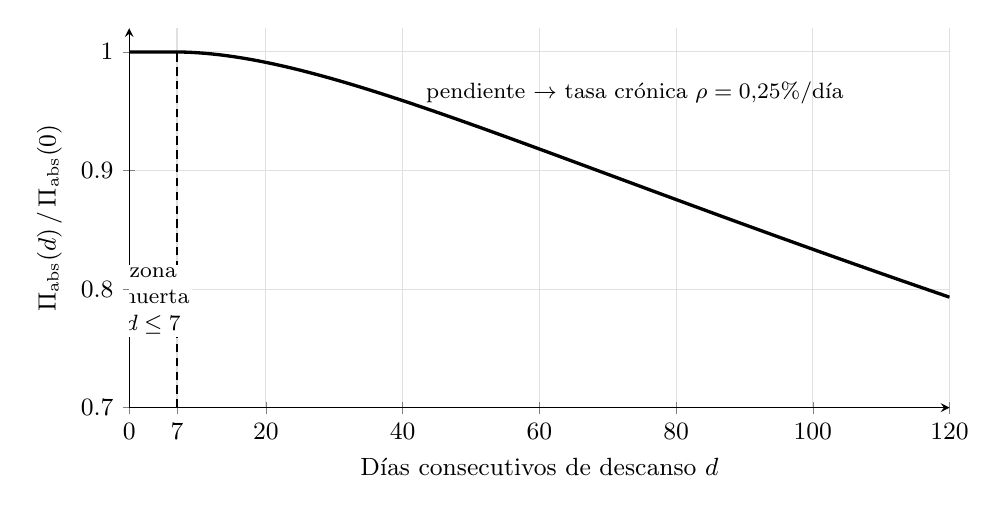
\begin{tikzpicture}
\begin{axis}[
  width=12cm, height=6.4cm,
  xlabel={D\'ias consecutivos de descanso $d$},
  ylabel={$\Pi_{\mathrm{abs}}(d)\,/\,\Pi_{\mathrm{abs}}(0)$},
  xmin=0, xmax=120, ymin=0.70, ymax=1.02,
  xtick={0,7,20,40,60,80,100,120}, ytick={0.7,0.8,0.9,1.0},
  grid=both, grid style={black!12},
  axis lines=left, tick label style={font=\small}, label style={font=\small},
]
\addplot[black, very thick] coordinates {(0,1.0) (1,1.0) (2,1.0) (3,1.0) (4,1.0) (5,1.0) (6,1.0) (7,1.0) (8,0.99988) (9,0.99966) (10,0.99932) (11,0.99889) (12,0.99836) (13,0.99774) (14,0.99703) (15,0.99624) (16,0.99538) (17,0.99443) (18,0.99342) (19,0.99234) (20,0.99119) (21,0.98999) (22,0.98872) (23,0.98741) (24,0.98604) (25,0.98462) (26,0.98315) (27,0.98164) (28,0.98009) (29,0.9785) (30,0.97687) (31,0.97521) (32,0.97351) (33,0.97178) (34,0.97003) (35,0.96824) (36,0.96643) (37,0.96459) (38,0.96273) (39,0.96085) (40,0.95895) (41,0.95702) (42,0.95508) (43,0.95312) (44,0.95115) (45,0.94916) (46,0.94716) (47,0.94514) (48,0.94312) (49,0.94108) (50,0.93903) (51,0.93697) (52,0.9349) (53,0.93283) (54,0.93074) (55,0.92865) (56,0.92656) (57,0.92446) (58,0.92235) (59,0.92024) (60,0.91812) (61,0.916) (62,0.91388) (63,0.91175) (64,0.90962) (65,0.90749) (66,0.90536) (67,0.90323) (68,0.90109) (69,0.89896) (70,0.89682) (71,0.89469) (72,0.89255) (73,0.89042) (74,0.88828) (75,0.88615) (76,0.88401) (77,0.88188) (78,0.87975) (79,0.87763) (80,0.8755) (81,0.87338) (82,0.87125) (83,0.86913) (84,0.86702) (85,0.8649) (86,0.86279) (87,0.86068) (88,0.85857) (89,0.85647) (90,0.85437) (91,0.85227) (92,0.85018) (93,0.84809) (94,0.846) (95,0.84392) (96,0.84184) (97,0.83977) (98,0.83769) (99,0.83563) (100,0.83356) (101,0.8315) (102,0.82945) (103,0.82739) (104,0.82535) (105,0.8233) (106,0.82126) (107,0.81923) (108,0.81719) (109,0.81517) (110,0.81314) (111,0.81113) (112,0.80911) (113,0.8071) (114,0.8051) (115,0.8031) (116,0.8011) (117,0.79911) (118,0.79712) (119,0.79514) (120,0.79316)};
\draw[black, densely dashed] (axis cs:7,0.70) -- (axis cs:7,1.0);
\node[fill=white, inner sep=1pt, font=\footnotesize, align=center] at (axis cs:3.5,0.79) {zona\\muerta\\$d\le 7$};
\node[font=\footnotesize, anchor=west] at (axis cs:42,0.965) {pendiente $\to$ tasa cr\'onica $\rho=0{,}25\%/$d\'ia};
\end{axis}
\end{tikzpicture}
\caption{Curva bif\'asica de desentrenamiento del od\'ometro $\Pi_{\mathrm{abs}}$, ecuaci\'on \eqref{eq:piabs}, normalizada al nivel previo al descanso. Durante los primeros $d_0{=}7$ d\'ias (zona muerta) no hay p\'erdida durable, pues la ca\'ida inicial corresponde a volumen plasm\'atico reversible. A partir de ah\'i la penalizaci\'on diaria crece de forma saturante (escala temporal $\tau_{\mathrm{dt}}{=}21$\,d) hacia la tasa cr\'onica $\rho$, produciendo un declive lento y casi lineal. Tras 120 d\'ias de inactividad el modelo retiene $\approx 79\%$ del nivel.}
\label{fig:piabs}
\end{figure}

\subsection{Marcadores biomecánicos: deriva del GCT y recuperación cardíaca}
\label{sec:biomech}

\paragraph{Deriva del tiempo de contacto (GCT drift).} Mide cuánto se degrada la técnica de carrera dentro de la sesión:
\begin{equation}
\mathrm{drift}_{\mathrm{GCT}} = \frac{\med\!\big(\mathrm{GCT}_{\text{20\% final}}\big) - \med\!\big(\mathrm{GCT}_{\text{20\% inicial}}\big)}{\med\!\big(\mathrm{GCT}_{\text{20\% inicial}}\big)},
\label{eq:gctdrift}
\end{equation}
donde $\med(\cdot)$ es la mediana del tiempo de contacto en el primer y último 20\% de la sesión. \textit{Interpretación:} un valor positivo significa que el pie pasa más tiempo en el suelo al final que al principio, señal de fatiga neuromuscular. En sesiones de intervalos se compara la primera con la última repetición de distancia comparable.

\paragraph{Recuperación de la frecuencia cardíaca.} Cuán rápido baja la FC tras un esfuerzo:
\begin{equation}
\mathrm{HRR}_{60} = \mathrm{HR}_{\mathrm{pico}} - \mathrm{HR}_{60\mathrm{s}},
\qquad
\mathrm{HR}(t) = \mathrm{HR}_{\mathrm{rec}} + \big(\mathrm{HR}_{\mathrm{pico}} - \mathrm{HR}_{\mathrm{rec}}\big)e^{-t/\tau_{\mathrm{HRR}}},
\label{eq:hrrec}
\end{equation}
donde $\mathrm{HR}_{\mathrm{pico}}$ es la FC al terminar el esfuerzo, $\mathrm{HR}_{60\mathrm{s}}$ la FC 60\,s después, $\mathrm{HR}_{\mathrm{rec}}$ la FC asintótica de reposo y $\tau_{\mathrm{HRR}}$ la constante de tiempo del descenso exponencial. \textit{Interpretación:} $\mathrm{HRR}_{60}$ (caída en un minuto) y $\tau_{\mathrm{HRR}}$ (rapidez del retorno completo) indican la reactivación parasimpática: descensos mayores y $\tau$ menores reflejan mejor recuperación \citep{stanley2013}. Solo se calcula si el esfuerzo previo alcanzó $\ge0{,}85\,\mathrm{HR}_{\max}$.
\newpage

% ======================================================================
\section{Supuestos y limitaciones}\label{sec:limits}
% ======================================================================

\subsection{Supuestos de validez}
\begin{enumerate}[leftmargin=1.4em,itemsep=2pt]
\item \textbf{Estacionariedad local de las líneas base.} Las ventanas de 42 y 90 días suponen que la distribución propia del atleta cambia lentamente. Tras cambios abruptos (lesión, enfermedad, salto de nivel) las líneas base quedan transitoriamente desalineadas.
\item \textbf{Constantes de literatura aplicables al individuo.} Las constantes de tiempo $\tau_g,\tau_h$ y los coeficientes del TRIMP se toman de la literatura general; su transferibilidad exacta a este atleta no se ha estimado y se asume razonable.
\item \textbf{Vigencia de los umbrales de dominio.} La separación aeróbico / alta intensidad depende de $v_{\mathrm{LT2}}$ y $\mathrm{HR@LT2}$, remedidos solo periódicamente; entre tests, un cambio real de umbral introduce un sesgo transitorio en el reparto de $g_{\mathrm{aer}}$ y $g_{\mathrm{hii}}$.
\item \textbf{Comparabilidad de la dinámica de carrera.} La deriva del GCT supone que las muestras del 20\% inicial y final son comparables en velocidad y terreno; en sesiones muy heterogéneas la comparación se restringe a tramos de distancia análoga.
\end{enumerate}

\subsection{Protocolo de análisis de sensibilidad y robustez}\label{sec:sensibilidad}

El sistema fija del orden de una docena de parámetros por diseño o por literatura, sin estimarlos de los datos. Esta decisión evita el mal condicionamiento, pero traslada el riesgo desde la \emph{varianza de estimación} hacia los \emph{grados de libertad del diseñador}: la elección manual de umbrales, ventanas y constantes. Mientras no se cuantifique a qué parámetros son sensibles las salidas, no puede afirmarse que esos valores estén justificados ni que el modelo sea robusto. Esta subsección fija el protocolo teórico con que debe evaluarse esa sensibilidad; no presenta resultados, sino el marco que los gobierna.

\paragraph{Principio rector.} Un parámetro fijo solo está justificado si (i) las salidas son robustas a su perturbación dentro de un rango razonable, en cuyo caso su valor exacto es irrelevante y puede fijarse sin culpa; o (ii) las salidas son sensibles a él, en cuyo caso debe medirse, citarse o someterse a especial cuidado, no elegirse a ojo. La sensibilidad es, por tanto, el criterio que separa los parámetros decorativos de los que de verdad gobiernan el modelo, y es condición previa a cualquier decisión de simplificación: ningún componente se elimina sin antes demostrar que su perturbación no mueve las salidas más allá del ruido.

\paragraph{Magnitudes objetivo.} El protocolo evalúa el desplazamiento de los descriptores de estado ante perturbaciones de los parámetros: el \emph{momentum} de forma $\Pi_{\mathrm{rel}}(t)$, el odómetro $\Pi_{\mathrm{abs}}(t)$ y los estados $g,h,\mathrm{TSB}$, junto con el reparto $g_{\mathrm{aer}},g_{\mathrm{hii}}$.

\paragraph{Diseño de perturbación.} Se adopta un barrido univariante (\emph{one-at-a-time}): cada parámetro se perturba aislando los demás en su valor base, y se re-corre la reconstrucción determinista completa desde el inicio del historial. El rango de perturbación es relativo ($\pm10\%$ y $\pm20\%$) para los parámetros multiplicativos, y absoluto para los que tienen escala física propia —en particular $\mathrm{HR}_{\mathrm{rest}}$, perturbada en $\pm1{,}5$ y $\pm3$\,bpm, coherente con la sensibilidad de $\sim2\%$ del TRIMP. El barrido univariante es deliberadamente conservador: detecta los efectos de primer orden con un número de corridas lineal en el número de parámetros; las interacciones entre los dos o tres parámetros dominantes se examinan después con un barrido conjunto reducido. El orden de prioridad sugerido, por impacto plausible, es $\mathrm{HR}_{\mathrm{rest}} \to (\tau_g,\tau_h) \to (\alpha,\rho,\tau_{\mathrm{dt}}) \to$ frontera del \emph{split} de dominio.

\paragraph{Métrica de desplazamiento.} Para hacer comparables descriptores de escalas distintas, el desplazamiento entre la corrida base y la perturbada se mide sobre los días comunes por el error cuadrático medio normalizado por la desviación estándar de la serie base. Un impacto agregado, suma ponderada explícita sobre los descriptores, ordena los parámetros.

\paragraph{Evidencia complementaria de estructura.} Junto al barrido, una comprobación de estructura informa decisiones de simplificación: la redundancia de $\Pi_{\mathrm{abs}}$ respecto de $g(t)$, evaluada por la correlación de rangos y por la fracción de varianza de $\Pi_{\mathrm{abs}}$ explicable linealmente por $g$. Una redundancia alta indicaría que el odómetro es, en lo esencial, una transformación monótona de la carga crónica acumulada, y que su complejidad añadida no se justifica.
% ======================================================================
\section{Discusión}
% ======================================================================

El diseño de Kairós representa una elección deliberada de \emph{sesgo bajo a costa de varianza controlada}: al renunciar a parámetros libres difíciles de estimar y al calibrar las señales derivadas intraindividualmente, el sistema sacrifica la ambición predictiva a cambio de descriptores interpretables y reproducibles. Esta postura es coherente con la evidencia de que los modelos impulso-respuesta completos son mal condicionados con datos individuales \citep{hellard2006}.

La decisión de desacoplar $\Pi_{\mathrm{rel}}$ (momentum de la trayectoria) de $\Pi_{\mathrm{abs}}$ (nivel durable acumulado) ilustra un principio recurrente: cada señal debe describir la dimensión que le corresponde. El primero responde a ``¿está subiendo la forma ahora?'' y el segundo a ``¿qué nivel se ha consolidado?''; mezclarlos confunde dinámica de corto plazo con adaptación de largo plazo.

Los marcadores biomecánicos intrasesión —deriva del GCT y recuperación cardíaca— complementan la familia de carga con información de \emph{cómo} se degrada y se recupera el atleta dentro del esfuerzo, sin entrar en la cadena EWMA que produce $g,h,\mathrm{TSB}$. Se reportan como observaciones independientes, no como insumos de la trayectoria de forma.

Las líneas de trabajo más críticas son (i) la remedición periódica de los umbrales de dominio ($v_{\mathrm{LT2}}$, $\mathrm{HR@LT2}$), que constituyen el ancla longitudinal más fiable frente a la deriva de las líneas base, y (ii) la ejecución del análisis de sensibilidad especificado en la Sección~\ref{sec:sensibilidad}, condición previa para justificar los parámetros fijos y para decidir, con evidencia, qué componentes pueden simplificarse sin pérdida.

% ======================================================================
\section{Conclusiones}
% ======================================================================

Kairós es un descriptor de estado fisiológico de propósito único que integra fisiología del ejercicio, biomecánica y teoría del entrenamiento bajo tres principios: descripción en lugar de predicción, calibración intraindividual y medición directa de los umbrales que separan dominios. Su salida es, para cada día, la carga y trayectoria de forma —$g$, $h$, $\mathrm{TSB}$, $\Pi_{\mathrm{rel}}$, $\Pi_{\mathrm{abs}}$ y los acumuladores de dominio $g_{\mathrm{aer}}, g_{\mathrm{hii}}$— complementada por dos marcadores biomecánicos intrasesión, la deriva del tiempo de contacto y la recuperación cardíaca. La formulación matemática —TRIMP de Banister, PMC en forma EWMA, índices de \emph{momentum} y de nivel durable— es interna y temporalmente coherente, y respeta una disciplina anti-circularidad que habilita su validación. Sus limitaciones (un solo sujeto, ausencia de \emph{ground truth}, dependencia de líneas base estacionarias y de umbrales remedidos) están explícitamente delimitadas. El documento permite comprender y reproducir conceptualmente el modelo sin acceso al código fuente.

% ======================================================================
\addcontentsline{toc}{section}{Referencias bibliográficas}
% ======================================================================
\begin{thebibliography}{99}
\setlength{\itemsep}{2pt}

\bibitem[Banister(1991)]{banister1991}
Banister, E.~W. (1991). Modeling elite athletic performance. En H.~J. Green, J.~D. McDougal y H.~Wenger (Eds.), \textit{Physiological Testing of Elite Athletes} (pp.~403--424). Human Kinetics.

\bibitem[Buchheit(2014)]{buchheit2014}
Buchheit, M. (2014). Monitoring training status with HR measures: Do all roads lead to Rome? \textit{Frontiers in Physiology, 5}, 73.

\bibitem[Calvert et al.(1976)]{calvert1976}
Calvert, T.~W., Banister, E.~W., Savage, M.~V., \& Bach, T. (1976). A systems model of the effects of training on physical performance. \textit{IEEE Transactions on Systems, Man, and Cybernetics, SMC-6}(2), 94--102.

\bibitem[Coyle et al.(1984)]{coyle1984}
Coyle, E.~F., Martin, W.~H., Sinacore, D.~R., Joyner, M.~J., Hagberg, J.~M., \& Holloszy, J.~O. (1984). Time course of loss of adaptations after stopping prolonged intense endurance training. \textit{Journal of Applied Physiology, 57}(6), 1857--1864.

\bibitem[Edwards(1993)]{edwards1993}
Edwards, S. (1993). \textit{The Heart Rate Monitor Book}. Fleet Feet Press.

\bibitem[Hellard et al.(2006)]{hellard2006}
Hellard, P., Avalos, M., Lacoste, L., Barale, F., Chatard, J.~C., \& Millet, G.~P. (2006). Assessing the limitations of the Banister model in monitoring training. \textit{Journal of Sports Sciences, 24}(5), 509--520.

\bibitem[Mujika \& Padilla(2000a)]{mujika2000a}
Mujika, I., \& Padilla, S. (2000). Detraining: Loss of training-induced physiological and performance adaptations. Part I: Short term insufficient training stimulus. \textit{Sports Medicine, 30}(2), 79--87.

\bibitem[Mujika \& Padilla(2000b)]{mujika2000b}
Mujika, I., \& Padilla, S. (2000). Detraining: Loss of training-induced physiological and performance adaptations. Part II: Long term insufficient training stimulus. \textit{Sports Medicine, 30}(3), 145--154.

\bibitem[Plews et al.(2013)]{plews2013}
Plews, D.~J., Laursen, P.~B., Stanley, J., Kilding, A.~E., \& Buchheit, M. (2013). Training adaptation and heart rate variability in elite endurance athletes: Opening the door to effective monitoring. \textit{Sports Medicine, 43}(9), 773--781.

\bibitem[Stanley et al.(2013)]{stanley2013}
Stanley, J., Peake, J.~M., \& Buchheit, M. (2013). Cardiac parasympathetic reactivation following exercise: Implications for training prescription. \textit{Sports Medicine, 43}(12), 1259--1277.

\end{thebibliography}

% ======================================================================
\appendix
\addcontentsline{toc}{section}{Anexo A. Glosario de s\'imbolos}
\section*{Anexo A. Glosario de s\'imbolos}\label{anexo:nomen}
% ======================================================================
Esta tabla re\'une todos los s\'imbolos empleados en la formulaci\'on del modelo, con su unidad y significado, para consulta independiente del cuerpo del informe.

\begin{small}
\begin{longtable}{@{}p{2.5cm}p{3.0cm}p{8.9cm}@{}}
\caption{Glosario de símbolos del modelo.}\label{tab:nomen}\\
\toprule
\textbf{Símbolo} & \textbf{Unidad} & \textbf{Qué representa} \\
\midrule
\endfirsthead
\multicolumn{3}{l}{\small\textit{(continuación de la Tabla \ref{tab:nomen})}}\\
\toprule
\textbf{Símbolo} & \textbf{Unidad} & \textbf{Qué representa} \\
\midrule
\endhead
\midrule \multicolumn{3}{r}{\small\textit{continúa\ldots}}\\
\endfoot
\bottomrule
\endlastfoot
\multicolumn{3}{@{}l}{\textit{Índices y operadores}}\\[2pt]
$t$ & --- & Día calendario. \\
$s$ & s & Instante dentro de una sesión (cada segundo). \\
$j,k$ & --- & Índices de día dentro de sumatorias y ventanas. \\
$\mu_W[\cdot],\,\sigma_W[\cdot]$ & --- & Media y desviación estándar sobre una ventana de $W$ días. \\
$z(\cdot)$ & --- & Z-score: desviación estandarizada respecto de la media propia. \\
$\clamp(x,a,b)$ & --- & Recorta $x$ al intervalo $[a,b]$ (lo limita por arriba y por abajo). \\
$\med(\cdot)$ & --- & Mediana de un conjunto de valores. \\
$\tanh(\cdot)$ & --- & Tangente hiperbólica; comprime cualquier número al rango $(-1,1)$. \\
$P_{99}(\cdot)$ & --- & Percentil 99 de un conjunto de valores. \\[4pt]
\multicolumn{3}{@{}l}{\textit{Frecuencia cardíaca y carga}}\\[2pt]
$\mathrm{HR}(s)$ & bpm & Frecuencia cardíaca (FC) instantánea. \\
$\mathrm{HR}_{\max}$ & bpm & FC máxima individual estimada. \\
$\mathrm{HR}_{\mathrm{rest}}$ & bpm & FC en reposo al despertar (ancla inferior de la reserva). \\
$\mathrm{HR}_{\mathrm{avg}}$ & bpm & FC media de una sesión. \\
$x(s)$ & --- (0--1) & Fracción de reserva de FC: posición de la FC entre reposo y máximo. \\
$L(t)$ & min-equiv & Carga de entrenamiento diaria (TRIMP). \\
$L_{\mathrm{Ban}}$ & min-equiv & TRIMP por el método de Banister. \\
$L_{\mathrm{aer}},L_{\mathrm{hii}}$ & min-equiv & Fracción aeróbica y de alta intensidad de la carga. \\
$b_0,b_1$ & --- & Coeficientes de la ponderación lactacidémica de Banister ($0{,}64$; $1{,}92$). \\
$v(s)$ & m\,s$^{-1}$ & Velocidad instantánea. \\
$v_{\mathrm{LT2}}$ & m\,s$^{-1}$ & Velocidad en el segundo umbral de lactato (de tests de escalón). \\
$\mathrm{HR@LT2}$ & bpm & FC en el segundo umbral de lactato. \\
$\phi(s),\theta$ & --- & Señal de intensidad del segundo $s$ y su umbral de separación de dominio. \\[4pt]
\multicolumn{3}{@{}l}{\textit{Modelo de forma (fitness--fatiga)}}\\[2pt]
$g(t)$ & min-equiv & Carga crónica (CTL): aptitud acumulada o \emph{fitness}. \\
$h(t)$ & min-equiv & Carga aguda (ATL): fatiga reciente. \\
$\mathrm{TSB}(t)$ & min-equiv & Balance de estrés o \emph{frescura} ($g$ menos $h$). \\
$\tau_g,\tau_h$ & días & Constantes de tiempo de $g$ (42) y $h$ (7): memoria de cada media. \\
$g_{\mathrm{aer}},h_{\mathrm{aer}},g_{\mathrm{hii}},h_{\mathrm{hii}}$ & min-equiv & Versiones por dominio (aeróbico / alta intensidad) de $g$ y $h$. \\
$r(j)$ & min-equiv/d & Tasa de rampa: cuánto supera la carga de hoy al CTL previo. \\
$\bar{r}_7(t)$ & min-equiv/d & Rampa promediada en 7 días (versión suavizada de $r$). \\
$z_{\mathrm{mom}}$ & --- & Z-score del \emph{momentum} de carga dentro de la ventana de 90 días. \\
$\sigma_{\min}$ & min-equiv/d & Piso de varianza que evita divisiones por valores casi nulos ($0{,}10$). \\
$\Pi_{\mathrm{rel}}(t)$ & --- ($-1$ a $1$) & Índice de forma relativo: dirección y fuerza del \emph{momentum}. \\
$\Pi_{\mathrm{abs}}(t)$ & --- & Nivel de corredor absoluto acumulado (``odómetro''). \\
$\alpha$ & --- & Escala de conversión rampa$\to$nivel en $\Pi_{\mathrm{abs}}$ ($5{,}0$). \\
$d$ & días & Número de días consecutivos de descanso. \\
$d_0$ & días & ``Zona muerta'' de descanso sin pérdida durable ($7$). \\
$\tau_{\mathrm{dt}}$ & días & Constante de tiempo del desentrenamiento ($21$). \\
$\rho$ & 1/día & Tasa crónica de pérdida diaria de nivel ($0{,}0025$). \\[4pt]
\multicolumn{3}{@{}l}{\textit{Marcadores biomecánicos intrasesión}}\\[2pt]
$\mathrm{GCT}$ & ms & Tiempo de contacto del pie con el suelo. \\
$\mathrm{drift}_{\mathrm{GCT}}$ & --- & Deriva (aumento relativo) del GCT dentro de la sesión. \\
$\mathrm{HRR}_{60}$ & bpm & Caída de FC en los 60\,s posteriores al pico de esfuerzo. \\
$\tau_{\mathrm{HRR}}$ & s & Constante de tiempo de la recuperación de FC. \\
$\mathrm{HR}_{\mathrm{pico}},\mathrm{HR}_{\mathrm{rec}}$ & bpm & FC al inicio de la recuperación y FC asintótica de reposo. \\
\end{longtable}
\end{small}


\end{document}